%CV for Samuel Runmark Thunell
% Last updated: November 17, 2022

\documentclass[a4paper,12pt]{article}

%PACKAGES
\usepackage{url}
\usepackage{parskip} 	

%other packages for formatting
\RequirePackage{color}
\RequirePackage{graphicx}
\usepackage[usenames,dvipsnames]{xcolor}
\usepackage[scale=0.9]{geometry}

%tabularx environment
\usepackage{tabularx}

%for lists within experience section
\usepackage{enumitem}

% centered version of 'X' col. type
\newcolumntype{C}{>{\centering\arraybackslash}X} 

%to prevent spillover of tabular into next pages
\usepackage{supertabular}
\usepackage{tabularx}
\newlength{\fullcollw}
\setlength{\fullcollw}{0.47\textwidth}

%custom \section
\usepackage{titlesec}				
\usepackage{multicol}
\usepackage{multirow}

%CV Sections inspired by: 
%http://stefano.italians.nl/archives/26
\titleformat{\section}{\large\scshape\raggedright}{}{0em}{}[\titlerule]
\titlespacing{\section}{0pt}{5pt}{5pt}

%for publications
\usepackage[style=authoryear,sorting=ynt, maxbibnames=2]{biblatex}

%Setup hyperref package, and colours for links
\usepackage[unicode, draft=false]{hyperref}
\definecolor{linkcolour}{rgb}{0,0.2,0.6}
\hypersetup{colorlinks,breaklinks,urlcolor=linkcolour,linkcolor=linkcolour}
\addbibresource{citations.bib}
\setlength\bibitemsep{1em}

%for social icons
\usepackage{fontawesome5}

%\usepackage{showframe}

\begin{document}

\pagestyle{empty} 

%Titles
\begin{minipage}{0.7\textwidth}
\begin{tabularx}{\linewidth}{@{}C @{}}
\Huge{Samuel Runmark Thunell} \\[7.5pt]
\href{https://smule.dev/}{\raisebox{-0.05\height}\faCode\ smule.dev} \ $|$ \ 
\href{https://linkedin.com/in/samuelrunmarkthunell}{\raisebox{-0.05\height}\faLinkedin\ samuelrunmarkthunell} \ $|$ \ 
\href{https://github.com/smuuule}{\raisebox{-0.05\height}\faGithub\ smuuule} \
\\
\href{mailto:samuel.runmark@gmail.com}{\raisebox{-0.05\height}\faEnvelope \ samuel.runmark@gmail.com} \ $|$ \ 
\href{tel:+46761692970}{\raisebox{-0.05\height}\faMobile \ +46.76.169.2970}  \\    
\end{tabularx} 
\end{minipage}
\hfill
\begin{minipage}{0.3\textwidth}
    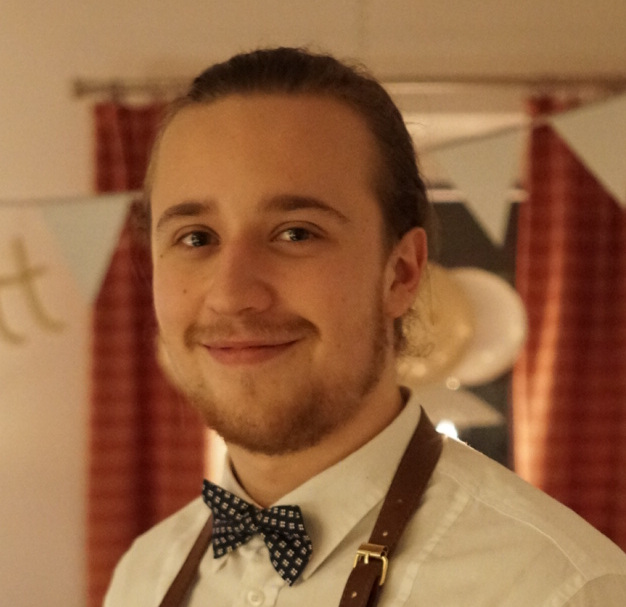
\includegraphics[scale=0.75]{DSC03993.JPG}
\end{minipage}


%Personal Introduction

\section{Who am I?}
I am a social, forward-facing, engaged student that never backs down from a challenge. I am right now studying for a Bachelor's Degree in Computer Science and Engineering at Chalmers University of Technology. In my free time, I'll spend time performing music, playing video games or hanging out with friends and family.

%Education
\section{Education}

\begin{tabularx}{\linewidth}{@{}l X@{}}	
2021 - present & Bachelor's student in Computer Science and Engineering at \textbf{Chalmers, Gothenburg} \hfill \\

2018 - 2021 & Technology Programme: Design and Product Development at \textbf{Åkrahäll, Nybro} \\ 
\end{tabularx}

%Experience
\section{Work Experience}

\begin{tabularx}{\linewidth}{ @{}l r@{} }
\textbf{Inventory Assistant, LogistikApoteket at \textbf{Tamro Sweden, Gothenburg}} & \hfill Jun 2023 - Aug 2023 \\[3.75pt]
\multicolumn{2}{@{}X@{}}{Tamro is the leading pharmaceutical logistics company in Sweden. Making sure that medicines and healthcare products meet expectations and to arrive on time brings a lot of bookkeeping and quality-testing. At Tamro, I learnt the importance of being structured and strategic in a stressful environment.}  \\
\end{tabularx}

\begin{tabularx}{\linewidth}{ @{}l r@{} }
\textbf{Machine Operator at \textbf{Smurfit Kappa, Nybro}} & \hfill Jun 2022 - Aug 2022 \\[3.75pt]
\multicolumn{2}{@{}X@{}}{The work in the production department of the Company gave me a good understanding of a machine's capabilities and shortcomings in a production line. A lot of the work meant precise adjustments to the machines settings and craved some mechanical engineering.}  \\
\end{tabularx}

\begin{tabularx}{\linewidth}{ @{}l r@{} }
\textbf{Park Supervisor at \textbf{Glasrikets Älgpark, Nybro}} & \hfill Jun 2020 - Aug 2020 \\[3.75pt]
\multicolumn{2}{@{}X@{}}{
    The supervisor position at the Moose Park consisted of maintaining a souvenir store and other public sites. It also gave me a great understanding of customer satisfaction and opportunities to hone my English.} \\
\end{tabularx}

%Volunteering Work
\section{Volunteering Work}

\begin{tabularx}{\linewidth}{ @{}l r@{} }
    \textbf{Treasurer at \textbf{DRUST/DBUS - Datateknologsektionen, Chalmers}} & \hfill May 2023 - present \\[3.75pt]
    \multicolumn{2}{@{}X@{}}{Being a Treasurer at the Student Division entailed managing finances and overseeing budgeting for sustainability. The work has learnt me a lot about how companies structure their digital bookkeeping and risk assessment.}  \\
    \end{tabularx}

\begin{tabularx}{\linewidth}{ @{}l r@{} }
\textbf{Commissioner at \textbf{DAG - Datateknologsektionen, Chalmers}} & \hfill May 2022 - April 2023  \\[3.75pt]
\multicolumn{2}{@{}X@{}}{I worked with bringing students of the CSE division closer to big tech companies; by helping them organize social events at Chalmers. I've learned a lot about companies in the Tech Industry and how to withhold professional client contact.}  \\
\end{tabularx}



%Skills

\section{Skills}

\begin{tabularx}{\linewidth}{@{}l X@{}}
\textbf{Programming Languages} &  \normalsize{Python, Java, C, Haskell, VHDL, JavaScript, Angular, react.js, C\#}\\
\textbf{Language Skills}  &  \normalsize{Swedish is my mother tongue, but I am also fluent in English.}\\
\textbf{Computer Enthusiast}  &  \normalsize{Computers hobbies as a young teenager gave me a loving understanding of both hard- and software} \\
\textbf{And more\dots}  &  \normalsize{Proficient in VC through Git, class B Driving Licence, Secretary for the Student Council of Åkrahäll, Adlerbertska Stipendiet (Scholarship).}
\end{tabularx}

\vfill

\end{document}